\section{Learning \& Training Dynamics}

\subsection*{Q: What is the role of Batch Normalization (BN) in training neural networks?}
\textbf{Batch normalization} normalizes the input of each layer to have zero mean and unit variance across a mini-batch. This reduces internal co-variate shift (changes in the distribution of layer inputs during training), speeds up convergence, and stabilizes activation distributions and gradients.

Mathematically, for a mini-batch \(B\) of size \(m\):
\[
\mu_B = \frac{1}{m} \sum_{i=1}^{m} x_i, \quad \sigma_B^2 = \frac{1}{m} \sum_{i=1}^{m} (x_i - \mu_B)^2
\]
\[
\hat{x}_i = \frac{x_i - \mu_B}{\sqrt{\sigma_B^2 + \epsilon}}, \quad y_i = \gamma \hat{x}_i + \beta
\]
where \(\epsilon\) is a small constant for numerical stability, and \(\gamma, \beta\) are learnable parameters.

\subsection*{Q: Why are learnable scale and shift parameters (\(\gamma, \beta\)) included in BN?}
BN restricts the distribution of outputs into the same fixed distribution (mean=0, variance=1), which prevents the network from learning the optimal scale and bias. These parameters allow the network to undo the normalization if necessary, preserving representational power after the input is normalized.

The parameters \(\gamma\) and \(\beta\) are learned during training:
\[
\gamma = \text{Var}[x]^{1/2}, \quad \beta = \mathbb{E}[x]
\]
This allows the network to recover the original distribution if it's optimal for the task.

\subsection*{Q: Where should BN be applied in a neural network?}
\textbf{Batch normalization} is typically applied after the affine transformation (like a linear or convolutional layer) and before the activation function such as ReLU. BN normalizes the pre-activation values which stabilizes the distribution before they pass through nonlinearities, which keeps gradients flowing smoothly during backpropagation. BN, typically, is not applied to the output layers.

The reasoning is that BN should normalize the inputs to activation functions, as activations like ReLU are sensitive to input distribution shifts. Normalizing pre-activations ensures the activation function receives well-distributed inputs.

\subsection*{Q: What are the limitations of BN with small batch sizes?}
Small batch sizes lead to noisy estimates of the mean and variance, which can destabilize training and degrade performance. This may result in issues such as batch-wise overfitting or jittery parameter updates. Additionally, Batch Normalization loses much of its regularization effect when batch statistics become unreliable. In practice, a "small batch" typically refers to fewer than 32 samples per batch per device.

The variance of the batch statistics scales as \(\text{Var}[\mu_B] = \frac{\sigma^2}{m}\), so smaller batches lead to noisier estimates.

\subsection*{Q: How does batch normalization work during inference?}
During inference, batch normalization (BN) uses the running averages of the mean and variance computed during training, rather than calculating them from the current batch of data. This ensures deterministic outputs regardless of batch size. However, the outputs during inference may differ slightly from those during training due to the shift from batch-wise statistics to running estimates.

The running statistics are updated during training as:
\[
\mu_{\text{running}} \leftarrow \alpha \mu_{\text{running}} + (1-\alpha) \mu_B
\]
\[
\sigma^2_{\text{running}} \leftarrow \alpha \sigma^2_{\text{running}} + (1-\alpha) \sigma^2_B
\]
where \(\alpha\) is typically 0.9 or 0.99.

\subsection*{Q: How do BatchNorm, LayerNorm, GroupNorm, and InstanceNorm compare?}
\begin{figure}[H]
	\centering
	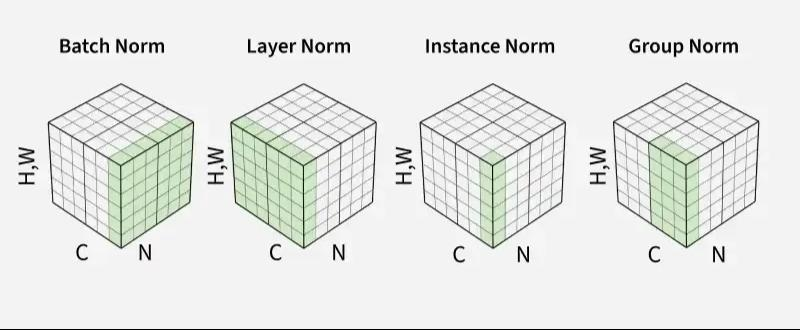
\includegraphics[width=0.8\textwidth]{norms.jpg}
	\caption{Source: \textit{https://www.geeksforgeeks.org/deep-learning/what-is-group-normalization/}}
\end{figure}
\begin{itemize}
	\item \textbf{Batch Normalization (BatchNorm)}: BatchNorm normalizes inputs across the batch dimension for each feature channel. It works well with large batch sizes and helps stabilize and accelerate training, but it can perform poorly with small batches and behaves differently during inference.
	\item \textbf{Layer Normalization (LayerNorm)}: LayerNorm normalizes across all feature dimensions within a single data sample. It is independent of batch size (robust for small batches) and is commonly used in architectures like Transformers and RNNs, but it tends to be less effective in convolutional neural networks.
	\item \textbf{Group Normalization (GroupNorm)}: GroupNorm divides channels into smaller groups and normalizes within each group. It performs consistently regardless of batch size and is particularly effective for convolutional models, though it requires tuning the number of groups (e.g., num groups=32).
	\item \textbf{Instance Normalization (InstanceNorm)}: InstanceNorm normalizes each individual sample and channel across spatial dimensions. It is widely used in style transfer applications as it helps remove instance-specific contrast information, but it may hurt performance in classification tasks where style information is important.
\end{itemize}

In summary, the choice of normalization method depends heavily on the task and batch size. For convolutional neural networks (CNNs) trained on large datasets like ImageNet, \textbf{BatchNorm} is the preferred choice. In scenarios with small batch sizes, such as object detection or segmentation, \textbf{GroupNorm} is typically more stable and effective. For natural language processing (NLP) and Transformer-based architectures, \textbf{LayerNorm} is widely used due to its batch-size independence. Finally, in style transfer or generative adversarial networks (GANs), \textbf{InstanceNorm} is favored for its ability to discard contrast and style-specific information.

\subsection*{Q: What are the differences between SGD and Adam?}
\textbf{SGD (Stochastic Gradient Descent)} uses a fixed or scheduled learning rate and is memory-efficient. The update rule is:
\[
\theta_{t+1} = \theta_t - \eta_t \nabla_\theta J(\theta_t)
\]
where \(\eta_t\) is the learning rate at step \(t\).

\textbf{Adam (Adaptive Moment Estimation)} adapts learning rates for each parameter and converges faster but may overfit. It maintains exponential moving averages of gradients and squared gradients:
\[
m_t = \beta_1 m_{t-1} + (1-\beta_1) \nabla_\theta J(\theta_t)
\]
\[
v_t = \beta_2 v_{t-1} + (1-\beta_2) (\nabla_\theta J(\theta_t))^2
\]
\[
\hat{m}_t = \frac{m_t}{1-\beta_1^t}, \quad \hat{v}_t = \frac{v_t}{1-\beta_2^t}
\]
\[
\theta_{t+1} = \theta_t - \frac{\eta}{\sqrt{\hat{v}_t} + \epsilon} \hat{m}_t
\]

Adam typically converges faster but may generalize less well than SGD with proper learning rate scheduling.

\subsection*{Q: What is the role of momentum in SGD?}
\textbf{Momentum} accumulates past gradients to smooth updates and accelerate convergence, especially in consistent gradient directions, and dampen oscillations caused by noisy gradients.

The momentum update rule is:
\[
v_{t+1} = \mu v_t - \eta \nabla_\theta J(\theta_t)
\]
\[
\theta_{t+1} = \theta_t + v_{t+1}
\]
where \(\mu\) is the momentum coefficient (typically 0.9).

Momentum helps in:
\begin{itemize}
	\item Accelerating convergence in consistent gradient directions
	\item Reducing oscillations in high-curvature regions
	\item Escaping local minima more effectively
\end{itemize}

\subsection*{Q: What are advanced optimization techniques beyond Adam?}
Several advanced optimizers have been developed to address Adam's limitations:

\begin{itemize}
	\item \textbf{AdamW}: Decouples weight decay from gradient-based updates, leading to better generalization:
	\[
	\theta_{t+1} = \theta_t - \frac{\eta}{\sqrt{\hat{v}_t} + \epsilon} \hat{m}_t - \lambda \theta_t
	\]
	
	\item \textbf{RAdam (Rectified Adam)}: Applies a warmup to the adaptive learning rate to prevent poor initialization:
	\[
	\rho_t = \rho_\infty - \frac{2t}{\beta_2^t}
	\]
	When \(\rho_t > 4\), RAdam uses the adaptive learning rate; otherwise, it falls back to SGD with momentum.
	
	\item \textbf{Lion}: A memory-efficient optimizer that uses sign-based updates:
	\[
	\theta_{t+1} = \theta_t - \eta \cdot \text{sign}(\beta_1 m_{t-1} + (1-\beta_1) \nabla_\theta J(\theta_t))
	\]
	
	\item \textbf{AdaBelief}: Adapts learning rates based on the belief in the observed gradients:
	\[
	s_t = \beta_2 s_{t-1} + (1-\beta_2) (\nabla_\theta J(\theta_t) - m_t)^2
	\]
\end{itemize}

\subsection*{Q: How can overfitting be reduced in machine learning models?}
Techniques include collecting more data (e.g., data augmentation), regularization (e.g., weight decay, dropout, L1/L2 regularization), early stopping, learning rate scheduling, model simplification, and model ensembling.

\textbf{Data Augmentation}: For images, techniques include rotation, scaling, cropping, color jittering, and mixup. For text, techniques include synonym replacement, back-translation, and EDA (Easy Data Augmentation).

\textbf{Regularization}: 
\begin{itemize}
	\item \textbf{Weight Decay (L2)}: Adds \(\frac{\lambda}{2} \|\theta\|_2^2\) to the loss
	\item \textbf{L1 Regularization}: Adds \(\lambda \|\theta\|_1\) to the loss, promoting sparsity
	\item \textbf{Dropout}: Randomly sets activations to zero during training
	\item \textbf{Early Stopping}: Monitors validation performance and stops when it degrades
\end{itemize}

\textbf{Learning Rate Scheduling}: Reduces learning rate over time:
\begin{itemize}
	\item \textbf{Step Decay}: \(\eta_t = \eta_0 \cdot \gamma^{\lfloor t/s \rfloor}\)
	\item \textbf{Cosine Annealing}: \(\eta_t = \eta_{min} + \frac{1}{2}(\eta_{max} - \eta_{min})(1 + \cos(\frac{t}{T}\pi))\)
	\item \textbf{One Cycle Policy}: Increases then decreases learning rate in a triangular pattern
\end{itemize}

\subsection*{Q: What is the difference between L1 and L2 regularization?}
\textbf{L1 regularization} adds absolute value penalties, leading to sparse models. The L1 penalty is \(\lambda \sum_{i} |\theta_i|\), which encourages many weights to become exactly zero, creating sparse models.

\textbf{L2 regularization} adds squared penalties, keeping weights small but non-zero. The L2 penalty is \(\frac{\lambda}{2} \sum_{i} \theta_i^2\), which shrinks weights toward zero but rarely makes them exactly zero.

Mathematically, the optimization problem becomes:
\[
\min_\theta J(\theta) + \lambda \|\theta\|_1 \quad \text{(L1)}
\]
\[
\min_\theta J(\theta) + \frac{\lambda}{2} \|\theta\|_2^2 \quad \text{(L2)}
\]

L1 is preferred when you want feature selection and interpretability, while L2 is better for preventing overfitting while maintaining model capacity.

\subsection*{Q: How does dropout work?}
\textbf{Dropout} is a regularization technique that randomly deactivates (or "drops") neurons during training with a specified probability. This prevents the network from becoming overly reliant on specific neurons and encourages redundancy in learned representations, which helps reduce overfitting.

During training, for each neuron, dropout applies:
\[
y = \frac{x \cdot \text{Bernoulli}(p)}{p}
\]
where \(p\) is the keep probability and \(\text{Bernoulli}(p)\) is a random binary mask.

During inference, dropout is disabled, and the output is scaled by \(p\) to maintain the expected value.

A high dropout rate increases regularization, which may cause the model to underfit if too much information is lost. Conversely, a low dropout rate provides weaker regularization, which may lead to overfitting if the model memorizes training data.

\subsection*{Q: Why does dropout improve generalization?}
\textbf{Dropout} acts like training many sub-networks and adds noise to the training process, which reduces overfitting and improves generalization.

Theoretical explanations include:
\begin{itemize}
	\item \textbf{Ensemble Effect}: Dropout trains an ensemble of \(2^n\) sub-networks (where \(n\) is the number of neurons)
	\item \textbf{Noise Injection}: Adds noise to the training process, making the model more robust
	\item \textbf{Feature Co-adaptation Prevention}: Prevents neurons from co-adapting to specific patterns
	\item \textbf{Regularization Effect}: Implicitly regularizes the model by constraining the effective capacity
\end{itemize}

\subsection*{Q: What are common activation functions and their pros/cons?}
\begin{figure}[H]
	\centering
	\includegraphics[width=0.8\textwidth]{activation.png}
	\caption{Source: \textit{https://blog.devops.dev/exploring-activation-functions-in-deep-learning-properties-derivatives-and-impact-on-model-7585aad8a757}.}
\end{figure}

\begin{itemize}
	\item \textbf{Sigmoid}: The sigmoid function is easy to interpret as it outputs values in (0, 1), but it may suffer from the vanishing gradient problem, especially at extreme input values.
	      \[
		      \sigma(x) = \frac{1}{1 + e^{-x}}
	      \]
	      Derivative: \(\sigma'(x) = \sigma(x)(1-\sigma(x))\), which approaches 0 for large \(|x|\).

	\item \textbf{Tanh}: The tanh function is zero-centered and ranges (-1, 1), which can help with optimization, but like the sigmoid function, it also experiences vanishing gradients.
	      \[
		      \tanh(x) = \frac{e^x - e^{-x}}{e^x + e^{-x}}
	      \]
	      Derivative: \(\tanh'(x) = 1 - \tanh^2(x)\).

	\item \textbf{ReLU}: The ReLU (Rectified Linear Unit) function is computationally efficient and helps create sparse representations, but it can suffer from the "dying ReLU" problem, where neurons become inactive.
	      \[
		      \text{ReLU}(x) = \max(0, x)
	      \]
	      Derivative: \(\text{ReLU}'(x) = \begin{cases} 1 & \text{if } x > 0 \\ 0 & \text{if } x \leq 0 \end{cases}\).

	\item \textbf{Leaky ReLU}: The Leaky ReLU addresses the dying ReLU issue by allowing a small, non-zero gradient when the unit is not active, improving learning stability.
	      \[
		      \text{LeakyReLU}(x) =
		      \begin{cases}
			      x        & \text{if } x \geq 0 \\
			      \alpha x & \text{if } x < 0
		      \end{cases}
	      \]
	      where \( \alpha \) is a small positive constant (typically \( \alpha = 0.01 \)).

	\item \textbf{GELU (Gaussian Error Linear Unit)}: A smooth approximation of ReLU that has become popular in transformer architectures:
	      \[
		      \text{GELU}(x) = x \cdot \Phi(x)
	      \]
	      where \(\Phi(x)\) is the cumulative distribution function of the standard normal distribution.

	\item \textbf{Swish}: A self-gated activation function that has shown strong empirical performance:
	      \[
		      \text{Swish}(x) = x \cdot \sigma(x)
	      \]
	      where \(\sigma(x)\) is the sigmoid function.

	\item \textbf{Softmax}: The softmax function converts logits into a probability distribution over classes, making it suitable for multi-class classification problems.
	      \[
		      \text{Softmax}(z_i) = \frac{e^{z_i}}{\sum_{j=1}^{C} e^{z_j}}
	      \]
	      where \( z_i \) is the logit for class \( i \), and \( C \) is the number of classes.
\end{itemize}

\subsection*{Q: When should you use Sigmoid vs Softmax?}
Use Sigmoid for binary or multi-label tasks. Use Softmax for mutually exclusive multi-class classification.

\textbf{Sigmoid} outputs independent probabilities for each class, suitable when:
\begin{itemize}
	\item Classes are not mutually exclusive (multi-label classification)
	\item Binary classification (single sigmoid unit)
	\item Output probabilities are independent of each other
\end{itemize}

\textbf{Softmax} ensures that all output probabilities sum to 1, suitable when:
\begin{itemize}
	\item Classes are mutually exclusive (single-label classification)
	\item You need a proper probability distribution
	\item Outputs should be dependent on each other
\end{itemize}

Mathematically, softmax ensures \(\sum_{i=1}^{C} \text{Softmax}(z_i) = 1\), while sigmoid allows \(\sum_{i=1}^{C} \sigma(z_i)\) to be any value between 0 and C.

\subsection*{Q: What is gradient flow and why is it important?}
\textbf{Gradient flow} refers to how gradients propagate backward through the network during training. Poor gradient flow can lead to vanishing or exploding gradients, making training difficult or impossible.

\textbf{Vanishing Gradients} occur when gradients become extremely small as they propagate backward, often in deep networks with sigmoid/tanh activations. The gradient update becomes:
\[
\frac{\partial L}{\partial \theta_l} = \frac{\partial L}{\partial \theta_L} \prod_{k=l}^{L-1} W_k^T \text{diag}(f'(\text{net}_k))
\]

If \(|f'(x)| < 1\) (as with sigmoid), the product approaches zero for deep networks.

\textbf{Exploding Gradients} occur when gradients become extremely large, often in recurrent networks. This can be addressed with gradient clipping:
\[
\text{if } \|\nabla_\theta J\| > \tau, \text{ then } \nabla_\theta J = \frac{\tau}{\|\nabla_\theta J\|} \nabla_\theta J
\]

\textbf{Techniques to improve gradient flow:}
\begin{itemize}
	\item Proper weight initialization (Xavier, He initialization)
	\item Batch normalization
	\item Residual connections (skip connections)
	\item Careful choice of activation functions
	\item Gradient clipping
\end{itemize}

\subsection*{Q: What are advanced weight initialization strategies?}
\textbf{Weight initialization} is crucial for training deep neural networks effectively. Poor initialization can lead to vanishing/exploding gradients or slow convergence.

\textbf{Xavier/Glorot Initialization}:
For a layer with \(n_{\text{in}}\) inputs and \(n_{\text{out}}\) outputs:
\[
W_{ij} \sim \mathcal{N}\left(0, \frac{2}{n_{\text{in}} + n_{\text{out}}}\right)
\]
This maintains variance of activations and gradients across layers.

\textbf{He Initialization}:
For ReLU activations:
\[
W_{ij} \sim \mathcal{N}\left(0, \frac{2}{n_{\text{in}}}\right)
\]
Accounts for the fact that ReLU sets half the activations to zero.

\textbf{Orthogonal Initialization}:
\[
W = U \Sigma V^T
\]
where \(U, V\) are orthogonal matrices. This helps with gradient flow in deep networks.

\textbf{Layer-sequential unit-variance (LSUV)}:
Initialize weights randomly, then adjust them so that each layer's output has unit variance on a batch of data.

\textbf{Mathematical intuition}:
For a layer with input \(x\) and output \(y = Wx + b\):
\[
\text{Var}[y_i] = \sum_{j=1}^{n_{\text{in}}} W_{ij}^2 \text{Var}[x_j]
\]

If weights are too large, variance explodes; if too small, it vanishes.

\subsection*{Q: What are curriculum learning and learning rate scheduling strategies?}
\textbf{Curriculum learning} presents training examples in a meaningful order, starting with simpler examples and gradually increasing difficulty.

\textbf{Mathematical formulation}:
For a curriculum function \(c(t)\) that determines difficulty at step \(t\):
\[
\text{Difficulty}(t) = c(t) \cdot \text{MaxDifficulty}
\]
where \(c(t)\) increases from 0 to 1 over training.

\textbf{Learning rate scheduling} adjusts the learning rate during training:

\textbf{Step Decay}:
\[
\eta_t = \eta_0 \cdot \gamma^{\lfloor t/s \rfloor}
\]
where \(s\) is the step size and \(\gamma\) is the decay factor.

\textbf{Cosine Annealing}:
\[
\eta_t = \eta_{\text{min}} + \frac{1}{2}(\eta_{\text{max}} - \eta_{\text{min}})\left(1 + \cos\left(\frac{t}{T}\pi\right)\right)
\]
where \(T\) is the total number of steps.

\textbf{One Cycle Policy}:
\[
\eta_t = \begin{cases}
\eta_{\text{max}} \cdot \frac{t}{T_{\text{warmup}}} & \text{if } t \leq T_{\text{warmup}} \\
\eta_{\text{max}} \cdot \left(1 - \frac{t - T_{\text{warmup}}}{T - T_{\text{warmup}}}\right) & \text{otherwise}
\end{cases}
\]

\textbf{Benefits}:
\begin{itemize}
	\item \textbf{Curriculum learning}: Faster convergence, better generalization
	\item \textbf{Learning rate scheduling}: Prevents overshooting, finds better minima
	\item \textbf{One cycle policy}: Combines benefits of high and low learning rates
\end{itemize}

\subsection*{Q: What are advanced regularization techniques beyond L1/L2 and dropout?}
\textbf{Advanced regularization} techniques address specific challenges in deep learning:

\textbf{Label Smoothing}:
Replaces hard labels with soft ones:
\[
y_{\text{smooth}} = (1 - \alpha) \cdot y + \alpha \cdot \frac{1}{K}
\]
where \(\alpha\) is the smoothing factor and \(K\) is the number of classes.

\textbf{Mixup}:
Creates new training examples by interpolating between pairs:
\[
x_{\text{mix}} = \lambda x_i + (1 - \lambda) x_j
\]
\[
y_{\text{mix}} = \lambda y_i + (1 - \lambda) y_j
\]
where \(\lambda \sim \text{Beta}(\alpha, \alpha)\).

\textbf{CutMix}:
Replaces rectangular regions of images:
\[
x_{\text{cutmix}} = M \odot x_i + (1 - M) \odot x_j
\]
where \(M\) is a binary mask and \(\odot\) is element-wise multiplication.

\textbf{Stochastic Depth}:
Randomly drops entire layers during training:
\[
y = \begin{cases}
f_l(x) & \text{with probability } p_l \\
x & \text{with probability } 1 - p_l
\end{cases}
\]

\textbf{ShakeDrop}:
Applies random scaling to residual connections:
\[
y = x + \alpha \cdot f(x)
\]
where \(\alpha \sim \text{Uniform}(0, 1)\).

\textbf{Mathematical benefits}:
\begin{itemize}
	\item \textbf{Label smoothing}: Prevents overconfidence, improves calibration
	\item \textbf{Mixup}: Increases effective dataset size, improves robustness
	\item \textbf{Stochastic depth}: Reduces overfitting, speeds up training
	\item \textbf{ShakeDrop}: Improves generalization through regularization
\end{itemize}
